\setcounter{section}{8}


\section{Lecture 9: Feb 8}


\subsection*{Last time}
\begin{itemize}
  \item Inference of SLR model
  \item Lab 1
\end{itemize}


\subsection*{Today}
\begin{itemize}
  \item SLR questions
  \item Multiple Linear Regression
\end{itemize}



\subsection*{Some questions to answer using regression analysis:}

\begin{enumerate}
  \item What is the meaning, in words, of $\beta_1$?\\
    \begin{pf}
    {\it Answer: }$\beta_1$ is the population slope parameter of the SLR model that represents the amount of increase in the mean of the response variable with a unit increase of the explanatory variable.
    \end{pf}
  \item True/False: (a) $\beta_1$ is a statistic (b) $\beta_1$ is a parameter (c) $\beta_1$ is unknown.\\
    \begin{pf}
    {\it Answer: } (a) False (b) True (C) True.  In reality, the true population parameters are almost never known.  However, in simulation studies, we do know them.
    \end{pf}
  \item True/False: (a) $\hat{\beta}_1$ is a statistic (b) $\hat{\beta}_1$ is a parameter (c)$\hat{\beta}_1$ is unknown\\
    \begin{pf}
    {\it Answer: } (a) True (b) False (C) False.  $\hat{\beta}_1$ is an estimate of the population parameter $\beta_1$.
    \end{pf}
  \item Is $\hat{\beta}_1 = \beta_1$ ?\\
    \begin{pf}
      {\it Answer: } No.  However, $\Expected{\hat{\beta}_1} = \beta_1$ 
    \end{pf}
\end{enumerate}

\subsection*{Multiple linear regression}
JF 5.2+6.2\\
\begin{center}
\underline{Multiple linear regression - an example}
\end{center}
An example on the prestige, education,  and income levels of $45$ U.S. occupations (Duncan's data):
\begin{center}
\begin{tabular}{ | c | c | c | c | c |}
\hline
 & income & education & prestige \\ 
\hline
accountant      & 62 &86 &82\\
pilot &72 &76 &83\\
architect & 75 &92 &90\\
author &55  &90 & 76\\
chemist   & 64 &  86 & 90\\
minister & 21 &  84 & 87\\
professor & 64 &  93 & 93\\
dentist & 80 & 100 & 90\\
reporter &   67 &  87 & 52\\
engineer & 72 &  86 & 88\\
lawyer & 76 &  98 & 89\\
teacher & 48 &  91 & 73\\
\hline
\end{tabular}
\end{center}
``prestige'' represents the percentage of respondents in a survey who rated an occupation as ``good'' or ``excellent'' in prestige,
``education'' represents the percentage of incumbents in the occupation in the 1950 U.S. Census who were high school graduates, 
and ``income'' represents the percentage of occupational incumbents who earned incomes in excess of \$3,500.

Using the \colorbox{shadecolor}{pairs} command in R, we can look at the pairwise scatter plot between the three variables as in Figure~\ref{fig:duncan_pair}.
\begin{figure}[H]
\begin{center}
  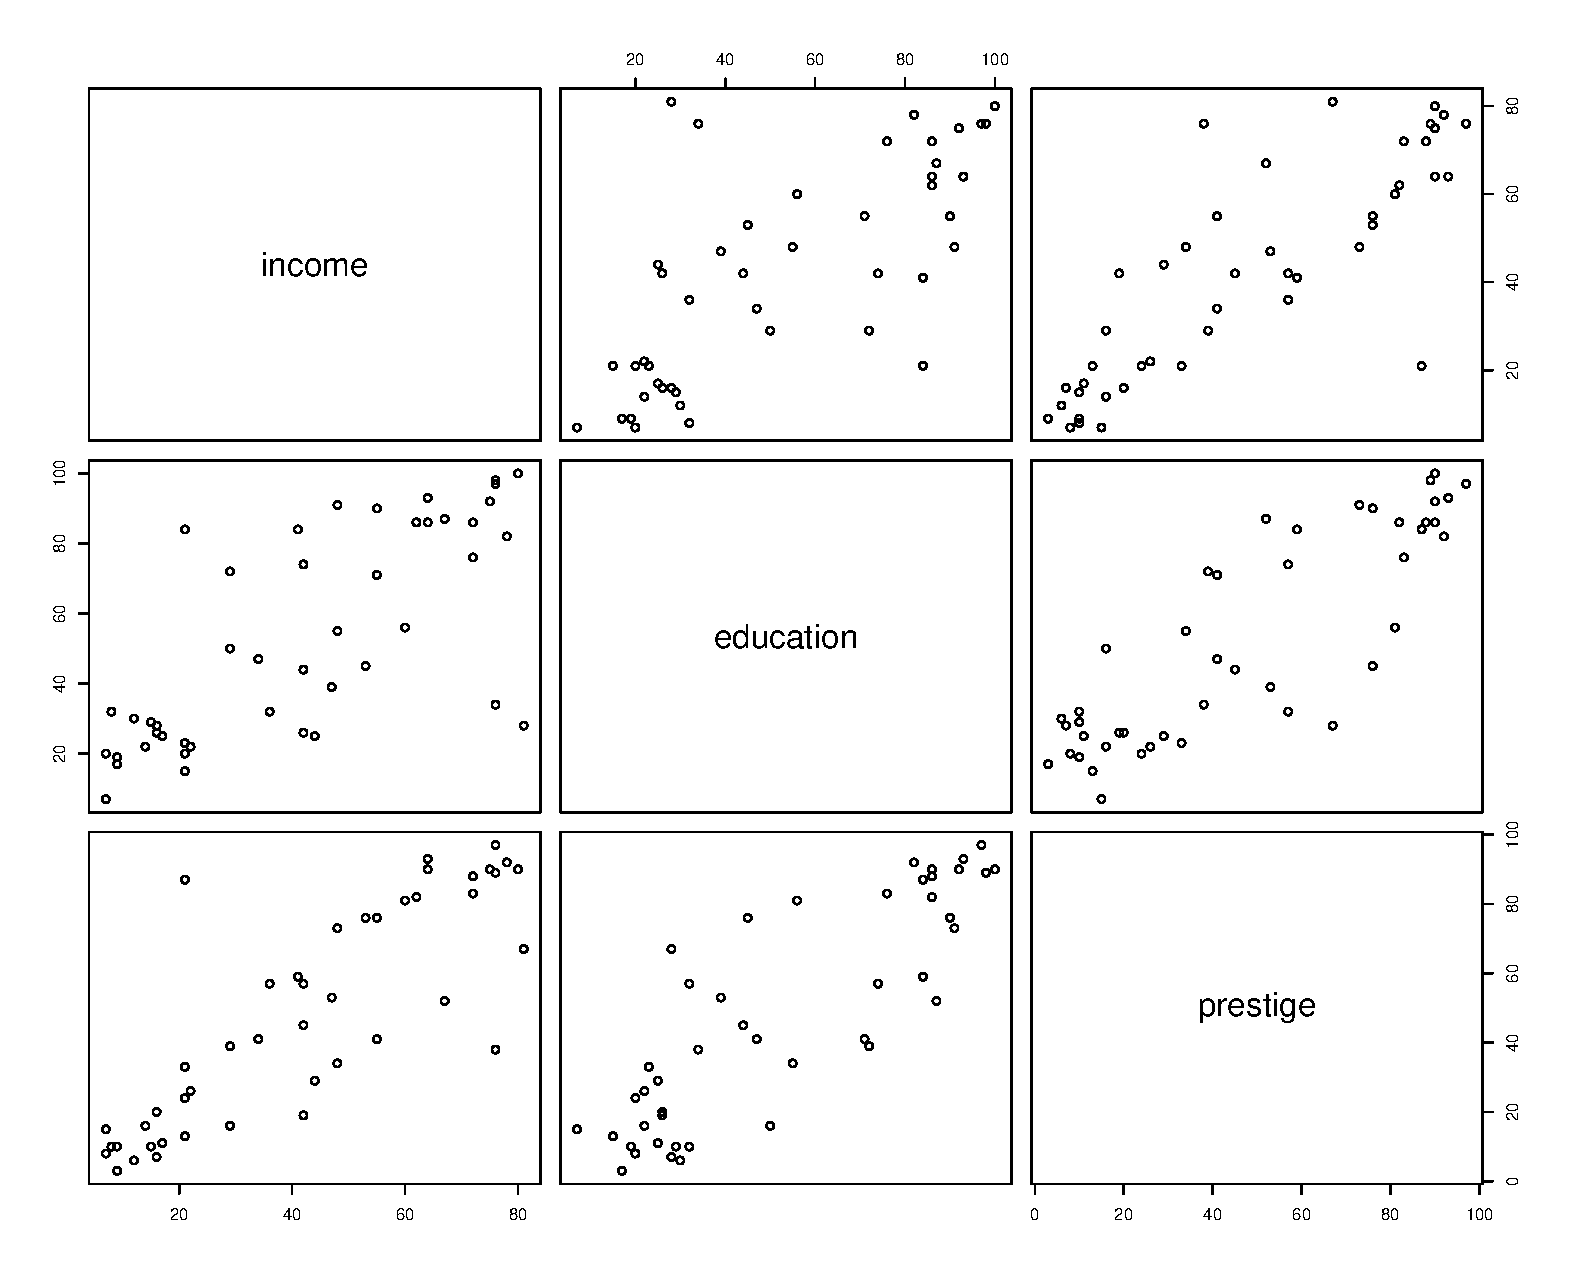
\includegraphics[width=0.8\textwidth]{Lecture9/Duncan_pairs.pdf}
  \caption{Scatterplot matrix for occupational prestige, level of education, and level of income of 45 U.S. occupations in 1950.}
  \label{fig:duncan_pair}
\end{center}
\end{figure}

Consider a regression model for the ``prestige'' of occupation $i$, $Y_i$, in which the mean of $Y_i$ is a linear function of two predictor variables $X_{i1} = income, X_{i2} = education$ for occupations $i = 1, 2,\dots, 45$:
$$
Y = \beta_0 + \beta_1 income + \beta_2 education + error
$$
or
$$
Y_i = \beta_0 + \beta_1 X_{i1} + \beta_2 X_{i2} + \epsilon_i
$$
or
$$
\begin{aligned}
Y_1 &= \beta_0 + \beta_1 X_{11} + \beta_2 X_{12} + \epsilon_1\\
Y_2 &= \beta_0 + \beta_1 X_{21} + \beta_2 X_{22} + \epsilon_2\\
\vdots &= \vdots\\
Y_{45} &= \beta_0 + \beta_1 X_{45,1} + \beta_2 X_{45,2} + \epsilon_{45}\\
\end{aligned}
$$

\subsection*{A multiple linear regression (MLR) model w/ $p$ independent variables}
Let $p$ independent variables be denoted by $x_1, \dots, x_p$.
\begin{itemize}
  \item Observed values of $p$ independent variables for $i^{th}$ subject from sample denoted by $x_{i1}, \dots, x_{ip}$
  \item response variable for $i^{th}$ subject denoted by $Y_i$
  \item For $i = 1, \dots, n$, MLR model for $Y_i$:
  $$
  Y_i = \beta_0 + \beta_1 x_{i1} + \beta_2 x_{i2} + \dots + \beta_p x_{ip} + \epsilon_i
  $$
  \item As in SLR, $\epsilon_1, \dots, \epsilon_n \distas{iid} N(0, \sigma^2)$
\end{itemize}

Least squares estimates of regression parameters minimize $SS[E]$:
$$
SS[E] = \sum\limits_{i = 1}^n (y_i - \beta_0 -  \beta_1 x_{i1} - \dots -\beta_p x_{ip})^2
$$

\begin{center}
\fbox{
$\hat{\sigma}^2 = \frac{SS[E]}{n - p - 1}$
}
\end{center}
%
Interpretations of regression parameters:
\begin{itemize}
  \item $\sigma^2$ is unknown \underline{error variance} parameter
  \item $\beta_0, \beta_1, \dots, \beta_p$ are $p + 1$ unknown regression parameters:
    \begin{itemize}
      \item $\beta_0$: average response when $x_1 = x_2 = \dots = x_p = 0$
      \item $\beta_i$ is called a \underline{partial slope} for $x_i$.  Represents mean change in $y$ per unit increase in $x_i$ {\it with all other independent variables held fixed}.
    \end{itemize}
\end{itemize}


\subsection*{Matrix formulation of MLR}
%
Let a ($1 \times (p + 1)$) vector for $p$ observed independent variables for individual $i$ be defined by 
$$
x_{i \cdot} = (1, x_{i1}, x_{i2}, \dots, x_{ip}).
$$
The MLR model for $Y_1, \dots, Y_n$ is given by
$$
\begin{aligned}
Y_1 &= \beta_0 + \beta_1 X_{11} + \beta_2 X_{12} + \dots + \beta_p X_{1p} + \epsilon_1\\
Y_2 &= \beta_0 + \beta_1 X_{21} + \beta_2 X_{22} + \dots + \beta_p X_{2p} + \epsilon_2\\
\vdots &= \vdots\\
Y_{n} &= \beta_0 + \beta_1 X_{n1} + \beta_2 X_{n2} + \dots + \beta_p X_{np} + \epsilon_{n}\\
\end{aligned}
$$
%
This system of $n$ equations can be expressed using matrices:
\begin{center}
\fbox{$\vecc{Y} = \vecc{X\beta} + \vecc{\epsilon}$}
\end{center}
%
where
\begin{itemize}
  \item $\vecc{Y}$ denotes a \underline{response vector} of size $n \times 1$
  \item $\vecc{X}$ denotes a \underline{design matrix} of size $n \times (p + 1)$
  \item $\vecc{\beta}$ denotes a vector of \underline{regression parameters} of size $(p + 1) \times 1$
  \item $\vecc{\epsilon}$ denotes an \underline{error vector} of size $n \times 1$
\end{itemize}
%
Here, the error vector $\vecc{\epsilon}$ is assumed to follow a multivariate normal distribution with variance-covariance matrix $\sigma^2 \vecc{I}_n$.
For individual $i$, 
$$
Y_i = x_{i \cdot} \beta + \epsilon_i.
$$
%
Some simplified expressions: ($\vecc{a}$ is a known $p \times 1$ vector)
\begin{subequations}
\begin{empheq}[box=\widefbox]{align*}
  \hat{\beta} &= (\vecc{X}\transpose \vecc{X})^{-1} \vecc{X}\transpose \vecc{Y}\\
  \Var{\hat{\beta}} &= \sigma^2 (\vecc{X}\transpose \vecc{X})^{-1}\\
                            &= \vecc{\Sigma}\\
  \reallywidehat{\sVar}{(\hat\beta)} &= MS[E] (\vecc{X}\transpose \vecc{X})^{-1}\\
                            &= \reallywidehat{\vecc{\Sigma}}\\
  \reallywidehat{\sVar}{(\vecc{a} \transpose \hat\beta)} &=\vecc{a} \transpose \reallywidehat{\vecc{\Sigma}} \vecc{a}\\
\end{empheq}
\end{subequations}
%
{\it Question: } what are the dimensions of each of these quantities?\\
\begin{itemize}
  \item $(\vecc{X}\transpose \vecc{X})^{-1}$ may be verbalized as `` x transposed x inverse''
  \item $\reallywidehat{\vecc{\Sigma}}$ is the estimated variance-covariance matrix for the estimate of the regression parameter vector $\vecc{\hat{\beta}}$
  \item $\vecc{X}$ is assumed to be of full {\it rank}.
\end{itemize}
%
Some more simplified expressions:
\begin{subequations}
\begin{empheq}[box=\widefbox]{align*}
  \hat{\vecc{Y}} 
  &= \vecc{X}\vecc{\hat{\beta}}\\
  &= \vecc{X} (\vecc{X}\transpose \vecc{X})^{-1} \vecc{X}\transpose \vecc{Y}\\
  &= \vecc{HY}\\
  \vecc{\hat{\epsilon}} 
  &= \vecc{Y} - \vecc{\hat{Y}}\\
  &= \vecc{Y} -  \vecc{X}\vecc{\hat{\beta}}\\
  &= (\vecc{I - H})\vecc{Y}\\
\end{empheq}
\end{subequations}
%
\begin{itemize}
  \item $\vecc{\hat{Y}}$ is called the vector of \underline{fitted} or \underline{predicted values}
  \item $\vecc{H} = \vecc{X} (\vecc{X}\transpose \vecc{X})^{-1} \vecc{X}\transpose$ is called the \underline{hat matrix}
  \item $\vecc{\hat{\epsilon}}$ is the vector of \underline{residuals}
\end{itemize}
%
For the Duncan's data example on income, education and prestige, with $p = 2$ independent variables and $n=45$ observations,
$$
\vecc{X} = \left[
\begin{tabular}{ccc}
1 & 62 &86\\
1 & 72 &76\\
\vdots&\vdots&\vdots\\
1 & 8 &  32\\
\end{tabular}
 \right]
$$
and
$$
\vecc{X}\transpose\vecc{X} = \left[
\begin{tabular}{ccc}
45 & 1884 &2365\\
1884 & 105148 &122197\\
2365 & 122197 &  163265\\
\end{tabular}
\right]
$$
$$
(\vecc{X}\transpose\vecc{X})^{-1} = \left[
\begin{tabular}{ccc}
0.10211 & -0.00085 &-0.00084\\
-0.00085 & 0.00008 &-0.00005\\
-0.00084 & -0.00005 &  0.00005\\
\end{tabular}
\right]
$$
$$
(\vecc{X}\transpose\vecc{X})^{-1} \vecc{X}\transpose \vecc{Y} = \left[
\begin{tabular}{c}
-6.0646629\\
0.5987328\\
0.5458339\\
\end{tabular}
\right] = ?
$$
$$
SS[E] = \epsilon \transpose \epsilon = (\vecc{Y} - \vecc{\hat{Y}})\transpose (\vecc{Y} - \vecc{\hat{Y}}) = 7506.7
$$
$$
MS[E] = \frac{SS[E]}{df} = \frac{7506.7}{45-2-1} = 178.73
$$
$$
\reallywidehat{\vecc{\Sigma}} = MS[E] (\vecc{X}\transpose\vecc{X})^{-1} = \left[
\begin{tabular}{ccc}
18.249481 & -0.151845008 & -0.150706025\\
-0.151845  & 0.014320275 & -0.008518551\\
-0.150706  & -0.008518551 &  0.009653582\\
\end{tabular}
\right]
$$
%


